\documentclass[margin=3mm]{standalone}
\usepackage{tikz}
\usetikzlibrary{shapes, arrows}

\tikzstyle{startstop} = [rectangle, rounded corners, minimum width=1cm, minimum height=1cm, text centered, draw=black, text=white, fill=black!80]
\tikzstyle{statement} = [rectangle, minimum width=1cm, minimum height=1cm, text centered, draw=black, fill=blue!20]
\tikzstyle{decision} = [rectangle, minimum height=1cm, text centered, draw=black, fill=yellow!30]
\tikzstyle{edge} = [thick, ->, >=stealth]

\begin{document}
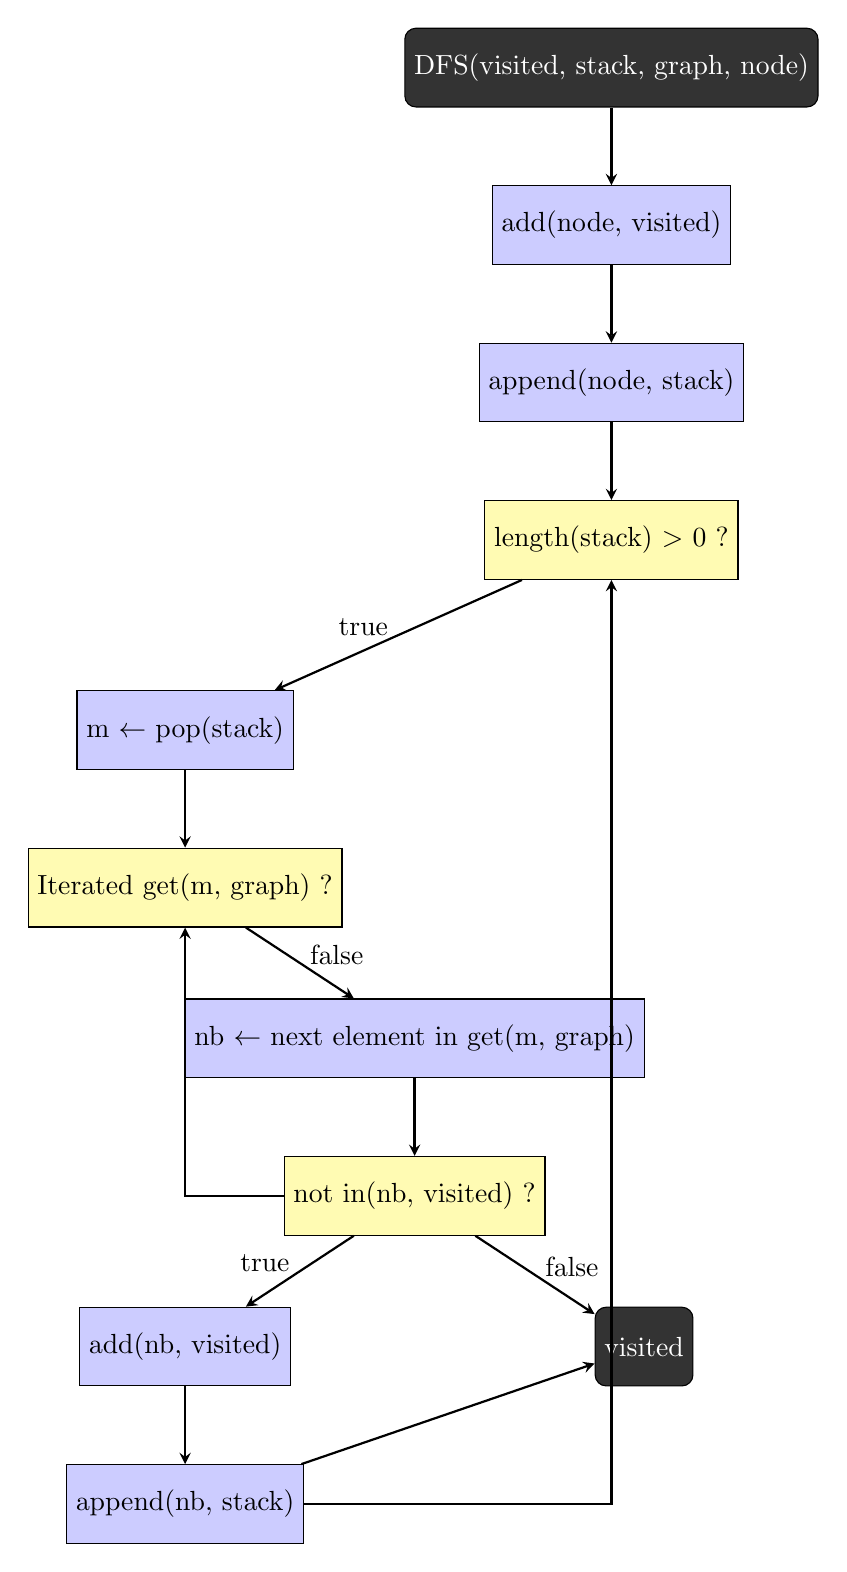
\begin{tikzpicture}[node distance=2cm]

\node (0) [startstop] {DFS(visited, stack, graph, node)};
\node (1) [statement, below of=0] {add(node, visited)};
\node (2) [statement, below of=1] {append(node, stack)};
\node (3) [decision, below of=2] {length(stack) $>$ 0 ?};
\node (4) [statement, yshift=-1cm, xshift=-4cm, below left of=3] {m $\gets$ pop(stack)};
\node (5) [decision, below of=4] {Iterated get(m, graph) ?};
\node (6) [statement, yshift=-0.5cm, xshift=1.5cm, below right of=5] {nb $\gets$ next element in get(m, graph)};
\node (7) [decision, below of=6] {not in(nb, visited) ?};
\node (8) [statement, yshift=-0.5cm, xshift=-1.5cm, below left of=7] {add(nb, visited)};
\node (9) [statement, below of=8] {append(nb, stack)};
\node (10) [startstop, yshift=-0.5cm, xshift=1.5cm, below right of=7] {visited};

\draw [edge] (0) -- (1);
\draw [edge] (1) -- (2);
\draw [edge] (2) -- (3);
\draw [edge] (3) -- node[anchor=east, yshift=0.1cm]{true} (4);
\draw [edge] (4) -- (5);
\draw [edge] (5) -- node[anchor=west, yshift=0.1cm]{false} (6);
\draw [edge] (6) -- (7);
\draw [edge] (7) -- node[anchor=west, yshift=0.1cm]{false} (10);
\draw [edge] (7) -| (5);
\draw [edge] (7) -- node[anchor=east, yshift=0.1cm]{true} (8);
\draw [edge] (8) -- (9);
\draw [edge] (9) -| (3);
\draw [edge] (9) -- (10);

\end{tikzpicture}
\end{document}